\documentclass[12pt]{article}

\usepackage{tikz}
\usepackage{graphicx}
\usepackage{caption}
\usepackage{subcaption}

\title{47510W Phoenix Horizon Programming}
\date{2024-2025}
\author{}

\graphicspath { {./figures} }

\begin{document}
 \maketitle
 \tableofcontents
 \newpage

\section*{Programming Environment}
\addcontentsline{toc}{section}{Programming Environment}
This section details the way in which we are managing our code for this robotics year.
\section{Version Control: Git}
For our version control system this year we have chosen the popular Git version control system. Git keeps track of each version of our code and also allows us to revert back if needed. We can also create multiple branches so we can work on a new part of the code without impacting the functioning code. Also, through the use of GitHub we can easily create a copy of our code and version history which lives in the web. Git also facilitates collaboration between team members working on the drive code. It is for these reasons that we have chosen Git for our version control for the 2024-2025 VRC competition.
\section{Robot API: Purdue PROS}
We have decided to use the Purdue PROS API to interface with our robot. We have chosen this API for it's superior performance and documentation over the standard VEX API, we also have more experience with PROS than VEXCODE. PROS also has great support for libraries. PROS does have one big drawback and that is the lack of suppoort for newer Vex equitment such as the AI Vison Sensor. Being a third party software, the PROS devolopment team does not have access to the VEX Software Delvelopment Kit(SDK).
\begin{figure}[h]
        \caption{API Comparison Table}
        \label{TABLE::API_COMP}
        \centering
        \begin{tabular}{c|c}
        PROS API & VEX API \\
        \hline
        Superior Performance & Can Be Sluggish \\
        Used Last Year & Used Two Years Ago(First Year) \\
        Readable Documentation & Some Docs Are Poorly Organized \\
        Third Party & Offical VEX \\
        Stable & New Fetaures Earlier \\
    \end{tabular}
\end{figure}


\section{Programming Libraries}
For this year we have decided to use the library LemLib. We have chosen this library becuase it is a popular library for the PROS API. Lemlib gives us esasy to use PID controllers and odometry algorithms such as point to point and boomerang. In accordance with the REC Code of Conduct, we have made sure that we understand the algorithm behind Lemlib. The notebook details each of these algorithms.

\section*{Algorithms for Programming}
\addcontentsline{toc}{section}{Algorithms for Programming}
This section of the notebook will detail the Algorithms that we are using for robot control.
\section{PID Controller Basics}
    A PID Controller (Proportional–Integral–Derivative Controller) is a control system that brings the system softly to a target, preventing overshoots and making for a more accurate program. PID controllers are used within our program to make more accurate turns and allow fine control over the amount the robot moves.

\subsection{How Does a PID Controller Work?} \label{howPID}
    Each term, $P$ $I$ $D$, each serve a specific role in creating and controlling the input which is used to reach the target. By adding up the values of the terms we get the input. We will analyze the function of each term individually.

\paragraph{P Term}
    The $P$ (Proportional) increases the input proportionally to the distance to the target. In other words, the farther you are from your target the larger the $P$ Term is. $P$ is the error, or distance from the target. We calculate the value of $P$ with the following formula.

    $$ P = T - M$$
    \begin{center}\em{Where T is target and M is the measured current value}\end{center}

    The $P$ Term is the primary way of tuning the PID and is always the first step. The specifics of tuning and how we tune each term will be discussed in a later section.

\paragraph{I Term}
    The $I$ (Integral) is the cumulative error. The $I$ term increases as the program runs and increases faster if farther away from the target. Which allows the controller to power over an obstacle, most often friction close to the target. We calculate the value of $I$ with the following formula.

    $$ I = I_0 + P$$
    \begin{center}\em{Where $I_0$ is the I term from the previous cycle, and P is the current error(The P term)}\end{center}

\paragraph{D Term}
    The $D$ (Derivative) is how fast the error is changing. The D term helps bring the controller out of a oscillating state caused by repeated overshoots, as are often induced by the $P$ term. We calculate the $D$ term with the following formula.

    $$D = P - P_0$$
    \begin{center}\em{Where P is the error(P term) and $P_0$ is the previous error (last P Term)}\end{center}

\paragraph{Putting It Together}
    To the get the input that we feed to our system, usually a motor for our purposes, we add together our three terms. Each of which multiplied by its tuning information. Tuning specifics will be covered in the next section. Our input formula is as follows.

    $$ R = P \cdot K_P + I \cdot K_I + D \cdot K_D$$
    \begin{center}
        \em{Where R is the output(or return), P I and D are the calculated values, and $K_P$ $K_I$ and $K_D$ are the tuning values}
    \end{center}

\subsection{Tuning A PID}
    For a PID to properly reach the target it must be tuned. Inadequate tuning can lead to failure to reach the target or aggressive oscillations. We tune a PID by changing tuning parameters, these parameters are called $K_P$ $K_I$ and $K_D$. The first step is to set all tuning parameters to 0. By setting a parameter to zero we can cut out their influence for the time being. As in the previous section we will look at the tuning of each term individually.

\paragraph{Tuning the $K_P$ Term}
    The first step to tuning a PID is to set the $K_P$ term. The first step to setting $K_P$ is to increases it until we get an overshoot and a settle either on the target or settles into an undershoot. If it settles on the target we are done with tuning and PID should be ready to use. If we settle into an undershoot we must move onto setting the $K_I$ term. If we overshoot or enter oscillations without settling we need to decrees the $K_P$ term.

\paragraph{Tuning the $K_I$ Term}
    The purpose of changing the $K_I$ term is to fix steady state error after the control settles. As a result of the behavior of the $I$ term to increases over time, it can add input to make the final push to the target even after the distance is not great enough for the $P$ term to have an effect. The $K_I$ does not need to be changed in all application. The $K_I$ term should be increased with caution because increasing it even by small amounts can introduce instability and overshoot.

\paragraph{Tuning the $K_D$ Term}
    The purpose of the $K_D$ term is to control oscillations in the system. We should change $K_D$ when the system has small but unacceptable oscillations. If the oscillations are large, it points to error in the $K_P$ term. Changing $K_D$ is often unnecessary in the context of robotics. We should change $K_D$ to refine out small errors when working with more precise systems such as driving and tuning. However systems which do not need to be super precise, like the speed of a flywheel, we can forgo tuning this term. Tuning of $K_D$ is a final refinement step to add extra stability or to counteract instability added by tuning $K_I$.

\newpage
\section{PID in Code}
    When using a PID for an actual application we can use the information described above to create a foundation, but we also need to add some extra parts to help with the imperfections of the real world. The change that must be made is to tell the program when it is ``Close Enough'' and it can stop. There is also the problem of feeding the input to the application. First we will look at the parts which are similar to the PID theory above.

\subsection{Initializing Variables and Setting Up}
    The first step to creating any new code system is to create an object (See the ``Overview of Object Oriented Programming'' to get information on this concept), and create variables we need. For now we will only create variables related to the theory and not the modifications required for a code implementation. This is all done in the header file (Also see the ``Overview of Programming Concepts'' for more information). So far, our code looks like the following.

    \begin{verbatim}
        in pid.hpp:

        class PID_OBJ
        {
            public:
                double p;
                double i;
                double d;
                double kp;
                double ki;
                double kd;

                double lastErr;

                PID_OBJ(double kp, double ki, double kd);

                double pidCalc(double target, double current);
                void reset(double target);
        };
    \end{verbatim}

    Let's break down that chunk of code a piece at a time. The first thing we see is the class declaration and the public keyword. These are explained in depth in the ``Overview of Object Oriented Programming''. For our purposes of explaining PID, they are unimportant. Then we see a list of variables all declared as floating point(decimal) values with double precision(hence the name 'double'). After that we declare 3 functions which we will look at in a moment. First, however, let us analyze the variables.

   \textbf{Variables.} We can see that we have many familiar variables which are reminiscent of the equations in the previous section. We also have a new variable \verb|double lastErr| which will keep track of what the error was during the last cycle of the control loop. If you recall from the section of the $D$ term, having access to the last error is important to the calculation of the term.

    \textbf{Functions.} Now we will look at the functions we have declared. The first function \verb|PID_OBJ| is a constructor and is called on the creation of a new PID. It takes three arguments, \verb|kp ki kd|, which should be familiar from both the section on tuning and our variables above. These arguments are how we will tune our system. The \verb|pidCalc| function does the operations described in section \ref{howPID}. Finlay the reset function allows us to reset the terms without creating a new PID. This is important between tasks to prevent interference. First we will look at the constructor and reset functions, then we will look at the \verb|pidCalc| function.

\subsection{Constructor and Reset Functions}
    The constructor and reset functions serve to initialize the PID before an external control loop. We will first look at the constructor.

    \textbf{Constructor.} The constructor serves to build a new PID object and set tuning information. The code within the constructor is as follows.

    \begin{verbatim}
    in pid.cpp:

        this->kp = kp;
        this->ki = ki;
        this->kd = kd;
    \end{verbatim}

    We are simply setting the passed values we saw in the header to internal values in the object which we can access later to do calculations with. This allows us to tune once. However, to use the PID multiple times we need to look at the rest function.

    \textbf{Reset.} The reset function sets the values of the PID to be ready for operation. It is absolutely necessary that this function is called before attempting to use the PID. We write the reset function like so.

    \begin{verbatim}
    in pid.cpp:

        this->p = 0;
        this->i = 0;
        this->d = 0;
        this->lastErr = target;
    \end{verbatim}

    We set each term to zero so the calculation has a clean slate. We set \verb|lastErr| to our target value because before the robot has moved, we can assume that the error(distance to the target) is equal to the target. This code could also be placed in the constructor, but this creates a ``Disposable PID'' which can only be used once. By moving the reset code into it's own function, we can reuse our PID.

\subsection{pidCalc Function}

    The \verb|pidCalc| function is the heart of our PID code. It calculates the P I and D terms and adds them together. Later we will also add code to this function to deal with the inconsistency of the robot. First we will look at calculating our terms. It is worth noting that target and current are passed in from the control outside the function, which will discuss later.
    \begin{verbatim}
        this->p = target - current;
        this->i += this->p;
        this->d = this->p - this->lastErr;
        this->lastErr = this->p;
    \end{verbatim}

    We see that we calculate the terms according to the formulas above just with different names. The symbol ``+='' after 'i' tells us that we should add the value on the right to the value on the left. We set \verb|lastErr| after we calculate 'd' because it is no longer relevant to this cycle and it will be equal to 'p' on the next cycle.

    After this we have a line to put the parts together.
    \begin{verbatim}
     return (this->p*this->kp)
        +(this->i*this->ki)+(this->d*this->kd);
    \end{verbatim}

    This line instructs the function to add the terms together after multiplying with their tuning information and return the sum as a result. We now have the foundations of a PID. Before we can implement it, we need to add code to deal with the real world.

\subsection{Dealing With Real World Inaccuracy}
    Sadly, the robot is not perfect and is not able to make zero tolerance turns. Our sensors also have some Inaccuracy that makes setting exact values impossible. Due to this fact we need to add code to call close enough when we are within a satisfactory zone. The first step is to add the following variables to our PID object.

    \begin{verbatim}
        double acceptableErr;
        bool isSettled;
        int acceptableCycles;
    \end{verbatim}

    Let's look at what each of these variables will do. The \verb|acceptableErr| variable will be set in the constructor and tells the PID how close is close enough. Like the tuning values, this needs to be set on a case by case basis for each application, however as a general rule values closer to zero will have more accurate results but require more precision. Values to close to zero may never settle. The \verb|isSettled| is a true or false value that will tell the control loop that we have settled and to move on. In a drive train context, the motors will be given stop commands after isSettled is set to true. Finally the \verb|acceptableCycles| tracks how many cycles we have been in range for.

    We start with checking if we are in an acceptable range.

    \begin{verbatim}
        if(fabs(p) <= acceptableErr)
    \end{verbatim}

    In this line we are saying that if the absolute value of our error is within the acceptable range we can move on. Otherwise, we go to the else condition which sets the acceptableCycles to zero. This else conditions means that we need to be in an acceptable range for a continuous span of time as opposed to passing through it a set number of times. The next line is the next step when we are within acceptable range.

    \begin{verbatim}
      if(this->acceptableCycles++ == 15)
        {
            this->isSettled = 1;
        }
    \end{verbatim}

    These lines add one to the acceptableCycles variable (reflecting the fact we just passed the acceptableCycles check) and then checks if we have at least 15 acceptable cycles. If we have reached this target we set is settled to True (represented by 1), otherwise we do nothing. Note that there is nothing special about 15. Any number will work there but larger numbers will be more accurate but take longer to settle.

    By putting these parts together we get code that is ready to handle the imperfection of the real world. Our full pidCalc function is as follows. (on next page)

    \begin{verbatim}
        in pid.cpp:

        this->p = target - current;
        this->i += this->p;
        this->d = this->p - this->lastErr;
        this->lastErr = this->p;

        if(fabs(p) <= acceptableErr)
        {
            if(this->acceptableCycles++ == 15)
            {
                this->isSettled = 1;
            }
        } else {
            acceptableCycles = 0;
        }
        return (this->p*this->kp)
            +(this->i*this->ki)+(this->d*this->kd);
    \end{verbatim}

    To use this function to run a system we need to create a control loop. We will use the autonomous tuning code as an example of this.

\subsection{PID Control Loop Example}
\paragraph{What does the control loop do?}
    By it's self the PID object is not able to affect the robot in any way. To put our code to work we need to add a control loop. This will take the outputs from the PID and give commands to the robot. We will show an example using autonomous turning code as this is a common use for PID.

\paragraph{Turning Example}

    We should first establish how we will track our current value. On the robot we have a sensor called the inertial sensor. This sensor tracks a number of values but the one we care about is rotation. Rotation tracks the how far we have rotated left or right in an angle. We will pass a value \verb|deg| to our turn function which will instruct the robot on how far it is to turn.

    Our first step is to calculate our starting value and reset the PID. We calculate our target with the following formula.
    $$ T = d + m $$
    \begin{center}
     \em{Where T is target, d is the value deg that we pass, and m is the measured current value}
    \end{center}

    After this we reset our PID, passing the target to the reset function. Our first two lines look as follows.

    \begin{verbatim}
        double target = deg + this->readInertialDeg();
        this->turPID.reset(target);
    \end{verbatim}

    Note that turPID is the PID that is set up with the tuning information regarding turning. Structure of the autonomous program will be discussed later.

    Next we create a loop which will calculate the current PID value and feed it to the motors. The code for that looks as follows.

    \begin{verbatim}
        while(true) {
            double calcVal = this->turPID.pidCalc(target,
                this->readInertialDeg());

            this->driveRight(calcVal);
            this->driveLeft(-calcVal);
    \end{verbatim}

    Note that the value we feed to the left motors is the opposite of that fed to the right motors. This is done so the robot will actually turn as opposed to going straight. We pass the value from the inertial sensor as the current measured value to the pidCalc function of the turPID (turn PID).

    Next we check if the PID has settled with a quick if statement, which is the following.
    \begin{verbatim}
     if(this->turPID.isSettled)
        {
            this->brake();
            return;
        }
    \end{verbatim}

    If the PID has settled the program tells the robot to brake and stop turning. After braking the loop ends and the robot has turned to the correct position. This concludes the section on the PID and we will now move onto optometry.


\pagebreak
\section{Basics of Optometry}
\subsection{What is Odometry}
    Odometry allows the robot to keep track of where it is on the field. In this imperfection, the robot keeps track of where it is relative to it's starting position. Odometry works by tracking the rotation of specific wheels and the heading of the robot.
    %should add odom wheel image here later :)

    By using the data from the wheels and sensors we are able to
    With Odometry we are able to tell the robot to go to a point as opposed to manually setting turns and movement. This allows for more precise programming that can remove errors in real applications.

\subsection{Odometry Sensors}
    Working with Odometry requires two kinds sensors. One to track the robot heading, the inertial sensor, and one to track the position of the odom wheels, the rotation sensor. We could also use a motor encoder, a comparison table of the two follows this.
    \begin{center}
        \begin{tabular}{c|c}
            Rotation Sensor & Motor Encoder \\
            \hline
            One Smart Motor Point & Two 3 wire ports \\
            More Precise & Less Precise \\
            Less Structure & More structure \\
            Center Screw Pivot & Must have makeshift pivot \\
        \end{tabular}

        We decided to use the rotation sensor because we benefit from the increased precision and better pivot.
    \end{center}

\subsection{Tracking Wheels}
We have decided to use 2.75in wheels for odometry. We chose this size because it is the smallest size we have. It is beneficial to use the smallest wheels available because the take of the least space. We also must measure the distance from the tracking center of the robot to the face of each tracking wheels. See Figure \ref{FIG::odom_offsets} below for how we measure tracking wheel offsets.

One final note about the sign of the distance. Based on the postion of the wheel relative to the tracking center we make the distance postive or negative. Front or left is positive and back or right is negative.

\def\wheelSize{1.5}
\begin{figure}[h]
 \caption{Measuring Odom Offsets}
 \label{FIG::odom_offsets}
 \centering
 \label{odom_offset_diagram}
 \begin{tikzpicture}
  \draw (0,0) rectangle (5,5);
  \draw (-0.5,3) rectangle (0,3+\wheelSize);
  \draw (-0.5,0.5) rectangle (0,0.5+\wheelSize);
  \draw (5.5,3) rectangle (5,3+\wheelSize);
  \draw (5.5,0.5) rectangle (5,0.5+\wheelSize);

  \draw[red, fill] (2.5,2.5) circle[radius=0.1];
  \node[red] at (2.5,2.9){Tracking Center};

  \draw (0.4,1) rectangle (0.9,1+\wheelSize);
  \draw [green,very thick](0.9,1.5) -- (2.5,1.5);
  \draw (2.5,1.2) -- (2.5,2.5);
  \node[green] at (1.7,1.2){Vertical};

  \draw (2.7,0.5) rectangle (2.7+\wheelSize, 1);
  \draw[blue,very thick](3.5,1) -- (3.5,2.5);
  \draw (2.5,2.5) -- (3.7,2.5);
  \node[rotate=270,blue] at (4.5,2){Horizontal};
  \node[red] at (2.5,4.5){Front};
 \end{tikzpicture}
\end{figure}


\pagebreak
\subsection{Determining Field Position}
\subsubsection{Finding $\Delta x$, $\Delta y$, and $\Delta\theta$}
The first step in determining the change in the field position is determining how much the robot heading changed. We use a continuous heading approach meaning that the heading does not reset after completing a rotation. Turing clockwise is repeated by a negative number and turning counterclockwise is represented by a positive number. We find the change in heading with the following formula. We choose the turning center of the robot for the tracking center because
$$
    \Delta \theta = \theta_1-\theta_0
$$
\textit{Where $theta_1$ is the current heading, $\theta_0$ was the last heading, and $\Delta \theta$ is the change in heading}

Next we must get the change on both odom wheels by using our rotation sensors. We can use the following formulas.

\textit{Let $degToIn(\theta)$ is a function which converts a value in degrees to a value in inches using the wheel diameter. (Wheel diameter is assumed in these formulas so is not listed.)}

See \ref{app_degToIn} for more information about degToIn including a formal derivation.
$$
    \Delta x = degToIn(R_{x_1} - R_{x_0})
$$
\textit{Where $\Delta x$ is the change in the $x$ direction. $R_{x_1}$ is the current position and $R_{x_0}$ is the last position of the wheel}
$$
    \Delta y = degToIn(R_{y_1} - R_{y_0})
$$
\textit{Where $\Delta y$ is the change in the $y$ direction. $R_{y_1}$ is the current position and $R_{y_0}$ is the last position of the wheel}

\subsubsection{Combining $\Delta x$, $\Delta y$, and $\Delta\theta$ in the current plane}
    For this section we define a variable robotOdomPos to store the odom position relative to the robot. This variable stores a (X,Y) coordinate.
\paragraph{When $\Delta\theta = 0$}
    we don't have to do any trigonometry at this step. We can simply store the x, y change into the variable. We can shorthand this with the following equation.
    $$ (\Delta x, \Delta y) = (X,Y)_{robotOdomPos} $$
\paragraph{When $\Delta\theta \neq 0$}\label{deltaneqtheta}
Our job becomes much more difficult if the robot heading changes during the movement. We must use the values from the tracking wheels and the inertial sensor readout to determine the actual change in position. The following is an explanation of this concept.

\subsubsection{Deriving Formulas to find $\Delta x$ and $\Delta y$ in the current plane when $\Delta\theta \neq 0$} \label{app_trighell}

Finding the $\Delta x$ and $\Delta y$ is done from the following diagrams.

\begin{figure}[h]\label{fig:xyfigs}
\centering
\caption{\textit{Given $C$, $X$, and $\theta$ find $y_{norm}$, $x_{norm}$ and $drift$ counterparts.}}
\begin{subfigure}{0.5\textwidth}

\centering
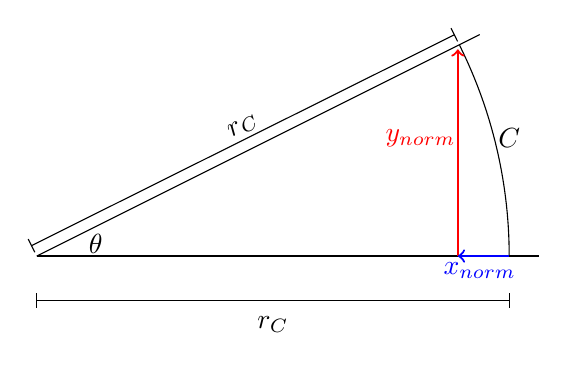
\begin{tikzpicture}[scale=0.75]
%main diagram
\draw (0,0) -- (8.5,0);
\draw(0,0) -- (7.5,3.75);
\draw (8,0) arc (0:26.5:8);
\node at (1,0.2){$\theta$};
\node at (8,2){$C$};
%r_c marks
\draw [shift={(0,-0.5)}](0,-0.25) -- (8,-0.25);
\draw [shift={(0,-0.5)}](0,-0.375) -- (0, -0.125);
\draw [shift={(0,-0.5)}](8,-0.375) -- (8, -0.125);
\node [shift={(0,-0.5)}] at (4,-0.5){$r_C$};

\draw [shift={(-0.2,0.4)}, rotate=26.5] (0,-0.25) -- (8,-0.25);
\draw [shift={(-0.2,0.4)}, rotate=26.5](0,-0.375) -- (0, -0.125);
\draw [shift={(-0.2,0.4)}, rotate=26.5](8,-0.375) -- (8, -0.125);
\node [rotate=30] at (3.5,2.2){$r_C$};

%xy marks

\draw[red,->, thick] (7.13,0) -- (7.13,3.5);
\node[red] at (6.5, 2){$y_{norm}$};
\draw[blue,->,thick] (8,0) -- (7.13,0);
\node[blue] at (7.5, -0.25){$x_{norm}$};
\end{tikzpicture}
\caption{Diagram of normal movement(not accounting drift)}
\label{norm_fig}
\end{subfigure}%
\begin{subfigure}{0.5\textwidth}

\centering
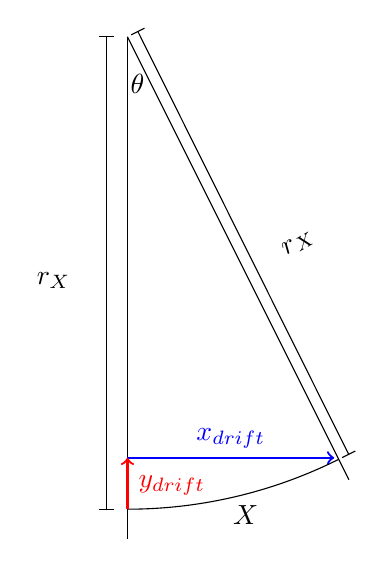
\begin{tikzpicture}[rotate=-90,scale=0.75]
%main diagram
\draw (0,0) -- (8.5,0);
\draw(0,0) -- (7.5,3.75);
\draw (8,0) arc (0:26.5:8);
\node at (0.8,0.17){$\theta$};
\node at (8.1,2){$X$};
%r_c marks
\draw [shift={(0,-0.1)}](0,-0.25) -- (8,-0.25);
\draw [shift={(0,-0.1)}](0,-0.375) -- (0, -0.125);
\draw [shift={(0,-0.1)}](8,-0.375) -- (8, -0.125);
\node [shift={(0,-0.1)}] at (4,-1.25){$r_X$};

\draw [shift={(-0.2,0.4)}, rotate=26.5] (0,-0.25) -- (8,-0.25);
\draw [shift={(-0.2,0.4)}, rotate=26.5](0,-0.375) -- (0, -0.125);
\draw [shift={(-0.2,0.4)}, rotate=26.5](8,-0.375) -- (8, -0.125);
\node [rotate=30] at (3.5,2.9){$r_X$};

%xy marks
\draw[blue,->, thick] (7.13,0) -- (7.13,3.5);
\node[blue] at (6.8, 1.75){$x_{drift}$};
\draw[red,->,thick] (8,0) -- (7.13,0);
\node[red] at (7.6, 0.75){$y_{drift}$};
\end{tikzpicture}
\caption{Diagram of drift movement}
\label{drift_fig}
\end{subfigure}
\end{figure}

For the purposes of this section we are assuming the tracking wheels are perfectly in the center of the robot. This is not possible in real robot design, but it simplifies the math. The corrections for real life applications are detailed in Section \ref{deltaneqtheta}. The $norm$ values do not account for drift and are determined from the y-wheel. $C$ is the value read from the sensor on the y-wheel. The $drift$ values are determined from the x-wheel. Likewise $X$ is the value read from the sensor on the x-wheel. We will first focus of the $norm$ values.
\paragraph{To find the norm values we must find $r_C$.} This value is the radius the the arc $C$, or the arc which the robot travels along(assuming no drifting). We use the formula for arc length to find the value $r_C$.

\centering
Formula for Arc Length
$$ s = \frac{\theta}{2\pi} (2\pi r) $$
Which can then be reduced by canceling $2\pi$:
$$ s = r\theta $$
\textit{Where $A$ is the arc length, $\theta$ is the internal angle of the arc in radians, and $r$ is the radius of the arc.}

We can substitute $C$ and $r_C$ and solve for $r_C$.
$$ C = \theta r_C $$
\textit{Dividing $theta$ from both sides.}
$$ \frac{C}{\theta} = r_C $$

\raggedright
We also add the distance from the the y-center of the robot to the wheel in actual application. We assume that distance is zero for theory purposes.

\paragraph{By using $r_C$} we can find values for $x_{norm}$ and $y_{norm}$. We can do this by using sine and cosine. Recall that on the unit circle $\sin\theta$ is the y value of a certain point and $\cos\theta$ is the x value of a certain point. Recognizing that Figure \ref{norm_fig} invokes the unit circle of radius $r_C$, we see that $y_{norm} = r_C \sin\theta$. We also find that $x_{norm} = -(r_C - r_C \cos\theta)$. We must subtract from the radius because we wish to find the $x$ distance from the start position to the current position, not from the origin to the start position. We also must make this value negative because the robot x is moving in the negative direction (Direction of movement is shown by the arrows in Figure \ref{norm_fig}). Finally we can factor out $r_C$ to simplify the formula for $x_{norm}$. So finally we come to the following two formulas for our $norm$ values.

\centering
$$y_{norm} = r_C \sin\theta$$
$$x_{norm} = -r_C(1-\cos\theta)$$

\raggedright
\pagebreak

\paragraph{To find the drift values,} we first must recognize that Figure \ref{drift_fig} is a rotation $90^{\circ}$ clockwise of Figure \ref{norm_fig}. The computation for $r_X$ is identical to that of $r_C$ just with values swapped for the different diagram. This means that we use $\cos$ for $y_{drift}$ and $\sin$ for $x_{drift}$. Contrary to the $norm$ values, neither term including $r_X$ is negative. This is seen in Figure \ref{drift_fig} as both arrows are pointing positive. So using the formulas from the $norm$ values, we derive the following formulas.
$$ x_{drift} = r_X \sin\theta$$
$$ y_{drift} = r_X (1-\cos\theta)$$

\paragraph{The last step of this process is to add the values together.} We find each $\Delta value$ in the current plane by adding the corresponding $norm$ and $drift$ values together.
$$ \Delta x = x_{norm} + x_{drift} $$
$$ \Delta y = y_{norm} + y_{drift} $$

We can the expand these values using our equations from the previous two subsections. Thus,
$$ \Delta x =  -r_C (1-\cos\theta) + r_X \sin\theta $$
$$ \Delta y =  r_C (1-\sin\theta) + r_X (1-\cos\theta) $$

\textit{Q.E.F}
\subsubsection{Rotating Into The Field's Plane}
We have now found the change in postion but it is from the robots previous frame of refrence.
We must rotate the point from the robots frame of refrence to the fields frame of refrence. We know the heading of the robot relative to the fields so we can use it to find the new point.
We will be refrencing the following diagram.

\begin{figure}
\caption{Point Rotation Diagram}
\label{FIG::PointRot}
\centering
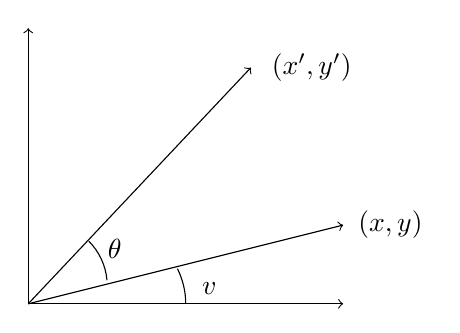
\begin{tikzpicture}
    %axes
    \draw [->](0,0) -- (0,3.5);
    \draw[->] (0,0) -- (4,0);
    %vectors
    \draw[->] (0,0) -- (4,1);
    \draw[->] (0,0) -- (2.828,3);
    \draw (2,0) arc (0:26.5:1);
    \draw (1,0.3) arc (5:45:0.8);
    %labels
    \node at (2.3, 0.2){$v$};
    \node at (1.1, 0.7){$\theta$};
    \node at (4.6,1){$(x,y)$};
    \node at (3.6,3){$(x',y')$};


\end{tikzpicture}
\end{figure}

\paragraph{To find the $x_1$}

\section{The pointToPoint function}

\section{Debugging}

\subsection{Brain Crashes 2024-8-19}
We ran into a runtime error during inital testing of our program. As soon as the program began it would crash. It gave us limited information, including a state printout. A state printout is where the program simply reports the current memory adresses on the CPU and runtime stack. See Figure \ref{FIG::statePrint} for an example.

By using a tool bundled with our cross complier we were able to locate possible error zones (Figure \ref{FIG::statePrint})
Both of these error zones were within library files, which we do not have easy access to.
The best course of action was decided to be to reintall Lemlib. This made no diffrence.
Still thinking that this was a problem with the library, we tried installing an old version of Lemlib. This also made no difference.
After talking with another team and collaborating on the debugging process, we found that the problem was with the order of intalization in the Robot class. It seems to of stemed from a misunderstanding in the use of intalizer lists.
We thought that the intializer list would begin at the top and step down, howevet it seems that
the intalizer list looks at the order of declarations in the class declaration and does it in that order. Due to the fact that we had declared chassis before it's component pieces, the program crashed. We fixed this by moving the chassis declaration to the bottom of the declration stack.
Correct and incorrect code can be found in Figure \ref{CODE::initOrderSimp}.
\begin{figure}
 \centering
 \caption{State Printout and Potential Error Areas}
 \label{FIG::statePrint}
 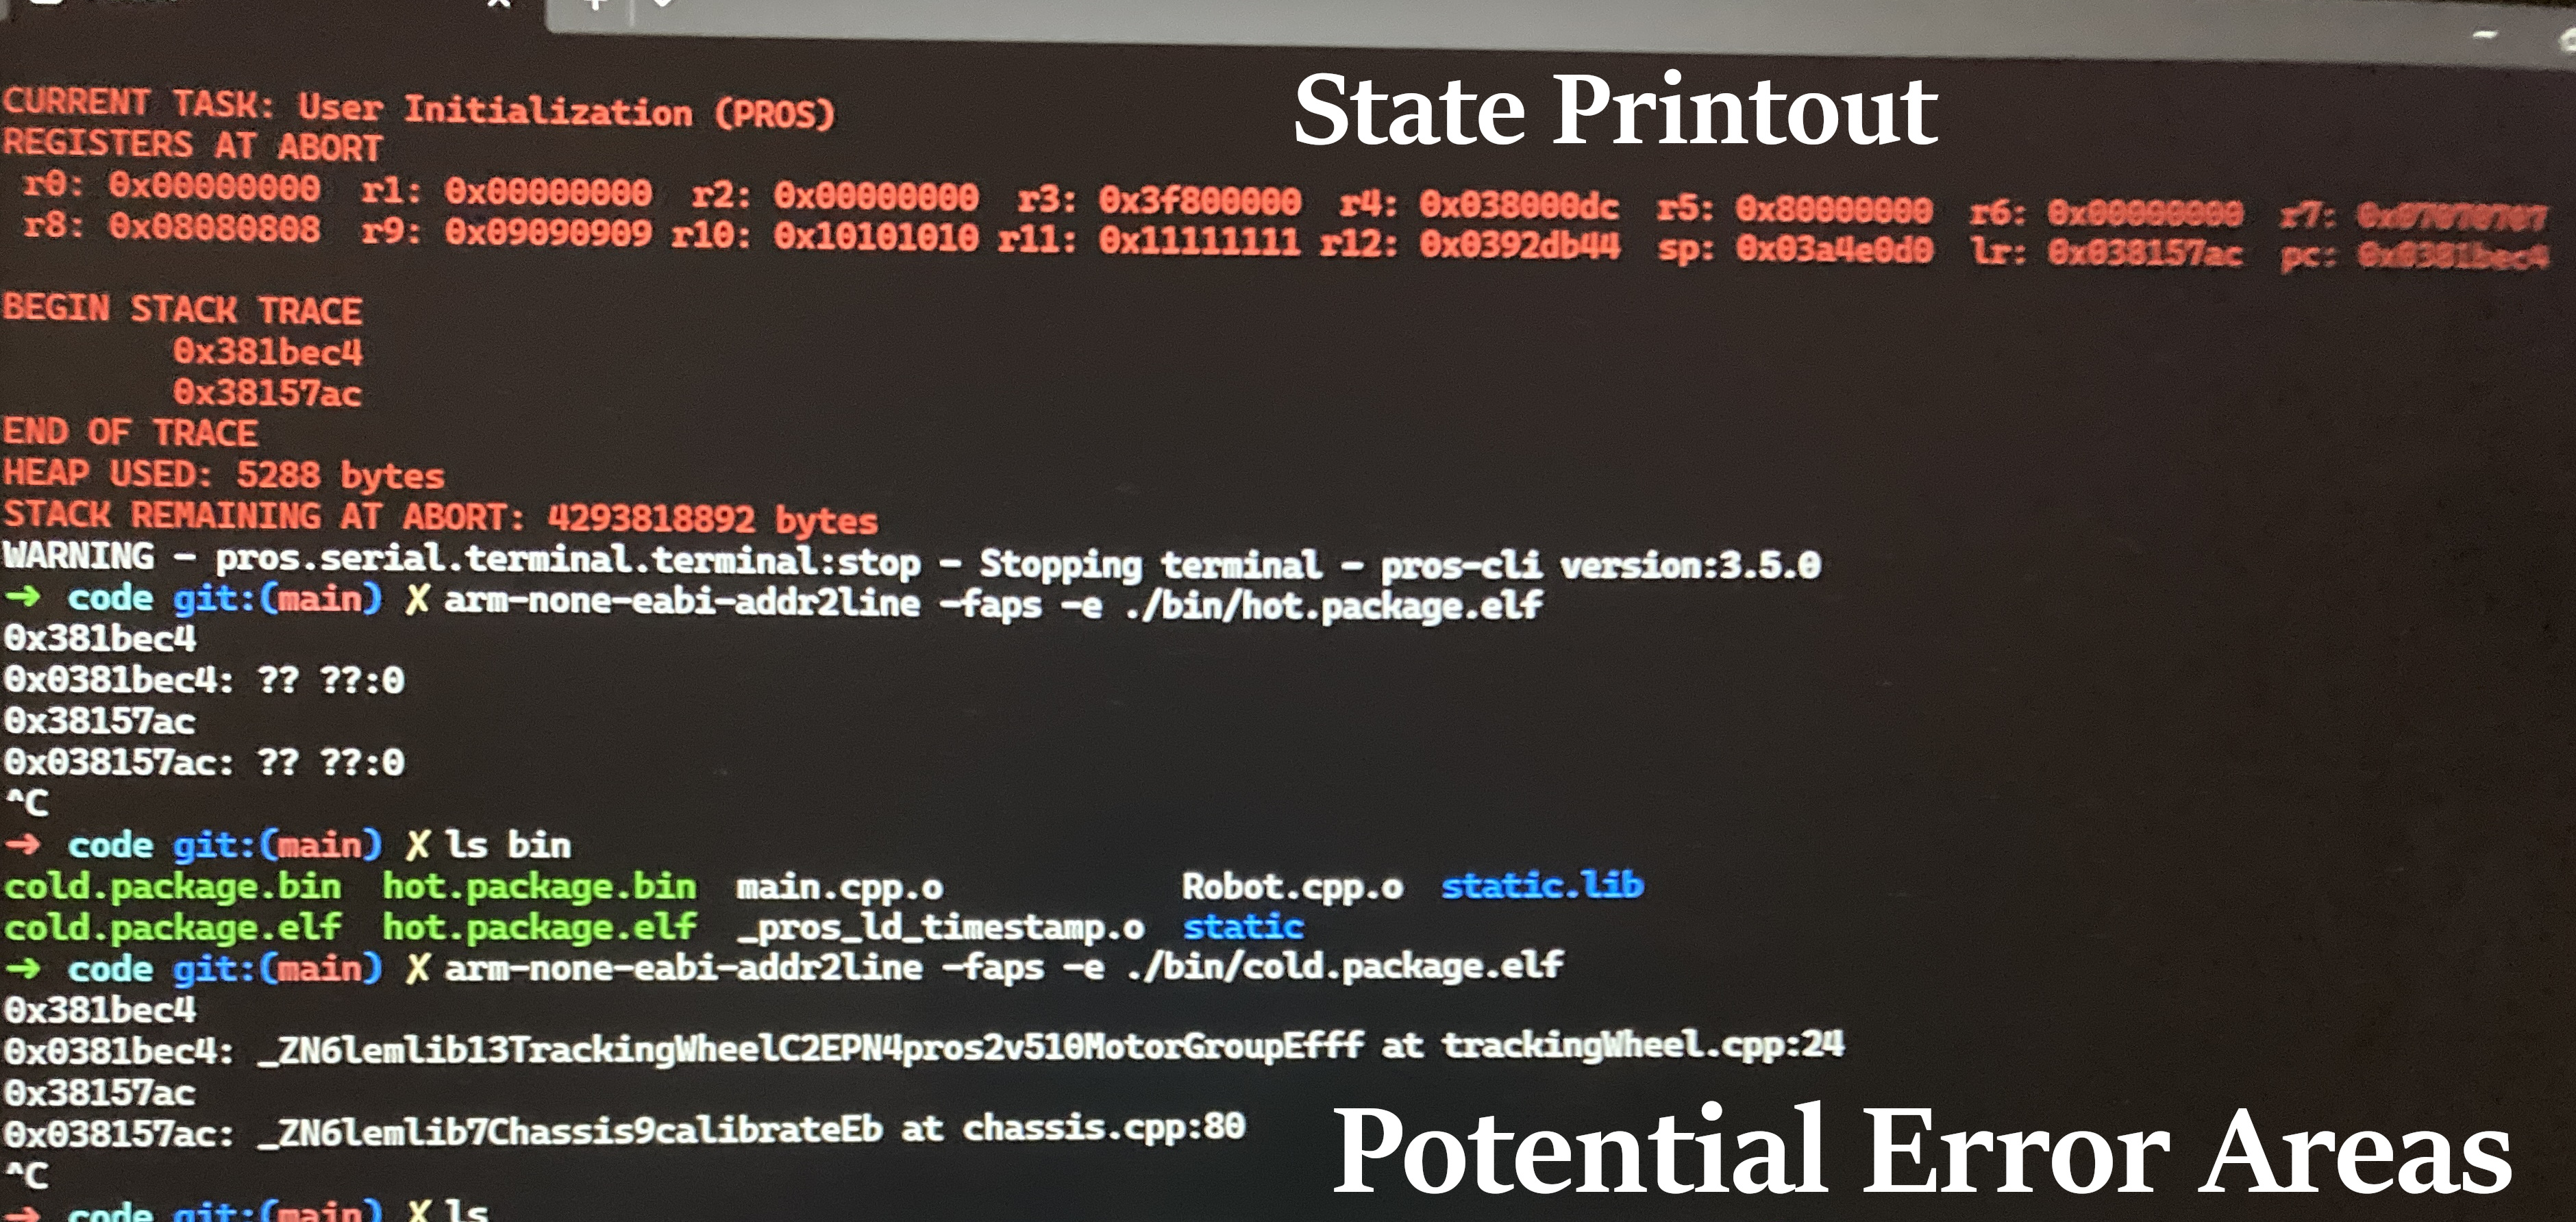
\includegraphics[scale=0.1]{statePrint}
\end{figure}

\pagebreak
\begin{figure}
\begin{subfigure}{0.5\textwidth}

\textit{Incorrect Intalization Order}
\begin{verbatim}
     class Robot
     {
        Chassis chassis;
        Drivetrain drivetrain;
        ControllerSet PIDS;
        Sensors odom_sensors;
     }
\end{verbatim}
\end{subfigure}%
\begin{subfigure}{0.5\textwidth}
\textit{Correct Intalization Order}
\begin{verbatim}
     class Robot
     {
        Drivetrain drivetrain;
        ControllerSet PIDS;
        Sensors odom_sensors;
        Chassis chassis;
     }

\end{verbatim}
\end{subfigure}
\caption{Initialization Order(Simplified)}
\label{CODE::initOrderSimp}
\end{figure}

% BEGIN APPENDIX
%
%
% BEGIN APPENDIX
\newpage
\appendix
\section*{Appendix}
\addcontentsline{toc}{section}{Appendix}
The appendix will detail background information and helper functions which are not specfic to robotics.
\section{Derivations for Helper Functions}
\subsection{Deriving the degToIn Function} \label{app_degToIn}
    The degToIn function uses basic circle geometry to convert the degrees a wheel rotates into the distance the wheel moves in inches using the wheel diameter. This function hinges on the principle that a wheel moves a distance equivalent to it's circumference for each full rotation. We define circumference with the equation.
    $$ C = d\pi $$
    \center\textit{Where $C$ is the circumference and $d$ is the diameter of the circle.}

    \raggedright
    This formula gives us the distance that the wheel moves if the wheel moves one rotation at a time. Sadly, though, in real life the wheel moves in fractional increments. We can represent this fractional rotation by multiplying the circumference by the same fraction. We find this fraction by dividing the measured valued by the amount of one rotation, in this case 360 degrees. We can use this fraction of a rotation to get the distance by multiplying it by the wheel circumference. So we use the following formula.
    $$ D = \frac{\theta^\circ}{360} \cdot C $$
    \center\textit{Where $D$ is the distance the wheel moved, $\theta^\circ$ is the degrees the wheel rotates, and $C$ is the circumference of the wheel.}

    \raggedright
    Finally we add this function into our code. We use M PI to put $\pi$ into the code. The function goes as follows.

    \begin{verbatim}
     double degToIn(double deg, double wheelDiam)
     {
         return (deg * (M_PI / 360.0)) * (wheelDiam);
     }
    \end{verbatim}

    \textit{Q.E.F}

    \pagebreak

\end{document}
